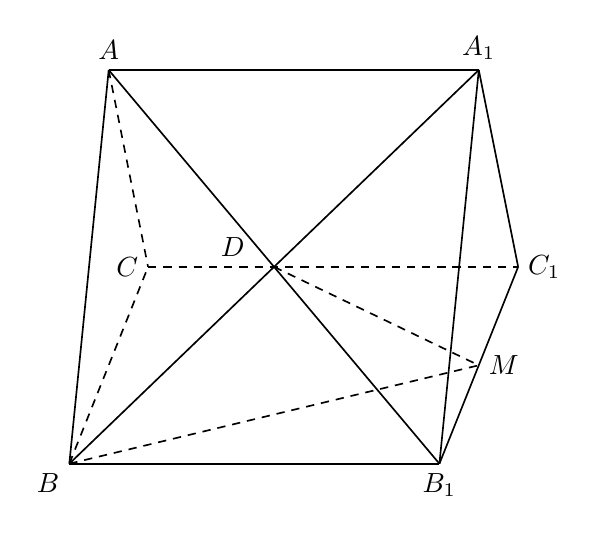
\begin{tikzpicture}[x=1cm,y=1cm,line width=0.6pt]
\coordinate (A) at (0.5,5);
\coordinate (A1) at (5.2,5);
\coordinate (B) at (0,0);
\coordinate (B1) at (4.7000000000,0.0000000000);
\coordinate (C) at (1.0,2.5);
\coordinate (C1) at (5.7000000000,2.5000000000);
\coordinate (D) at (2.6000000000,2.5000000000);
\coordinate (M) at (5.2000000000,1.2500000000);
% prism outline solid
\draw[draw=black,solid] (A) -- (A1);
\draw[draw=black,solid] (A) -- (B);
\draw[draw=black,solid] (B) -- (B1);
\draw[draw=black,solid] (A1) -- (C1);
\draw[draw=black,solid] (A1) -- (B1);
\draw[draw=black,solid] (B1) -- (C1);
% side-face diagonals through D
\draw[draw=black,solid] (A) -- (B1);
\draw[draw=black,solid] (B) -- (A1);
% hidden dashed edges
\draw[draw=black,dashed,dash pattern=on 3pt off 2.5pt] (A) -- (C);
\draw[draw=black,dashed,dash pattern=on 3pt off 2.5pt] (C) -- (C1);
\draw[draw=black,dashed,dash pattern=on 3pt off 2.5pt] (B) -- (C);
\draw[draw=black,dashed,dash pattern=on 3pt off 2.5pt] (C) -- (D);
\draw[draw=black,dashed,dash pattern=on 3pt off 2.5pt] (D) -- (M);
\draw[draw=black,dashed,dash pattern=on 3pt off 2.5pt] (B) -- (M);
% labels with clearance
\node[font=\normalsize,anchor=south,xshift=0pt,yshift=0pt] at (A) {$A$};
\node[font=\normalsize,anchor=south,xshift=0pt,yshift=0pt] at (A1) {$A_{1}$};
\node[font=\normalsize,anchor=north east,xshift=0pt,yshift=0pt] at (B) {$B$};
\node[font=\normalsize,anchor=north,xshift=0pt,yshift=0pt] at (B1) {$B_{1}$};
\node[font=\normalsize,anchor=east,xshift=0pt,yshift=0pt] at (C) {$C$};
\node[font=\normalsize,anchor=west,xshift=0pt,yshift=0pt] at (C1) {$C_{1}$};
\node[font=\normalsize,anchor=east,xshift=-7pt,yshift=7pt] at (D) {$D$};
\node[font=\normalsize,anchor=west,xshift=0pt,yshift=0pt] at (M) {$M$};
\end{tikzpicture}
